\documentclass[a4paper,11pt]{article}
\usepackage[utf8]{inputenc}
%\usepackage{fullpage}
\usepackage{listings}
\usepackage{color}
\usepackage{url}
\usepackage{alltt}
\usepackage{multicol}
\usepackage{fancyhdr}
\usepackage{amsmath}
\usepackage{bussproofs}
\usepackage{comment}
\usepackage{hyperref}
\usepackage[lighttt]{lmodern}
\usepackage{graphicx}

\renewcommand{\familydefault}{\sfdefault} % change to sans serif font

\newcommand{\seq}{\vdash}	% the sequent sign
\newcommand{\impl}{\supset} %logical connectives: implies, not, and, or
\renewcommand{\lnot}{\neg}
\renewcommand{\land}{\wedge}
\renewcommand{\lor}{\vee}
\newcommand{\sklabel}[2]{\langle#1\rangle^{#2}}

%Commands for constructing proof trees with bussproofs. See the chapter on the LK system for examples.
\newcommand{\UnaryInfCm}[1]{\UnaryInfC{$#1$}}
\newcommand{\BinaryInfCm}[1]{\BinaryInfC{$#1$}}
\newcommand{\RightLabelm}[1]{\RightLabel{$#1$}}
\newcommand{\AxiomCm}[1]{\AxiomC{$#1$}}

% Normal text in math mode ("math text")
\newcommand{\mt}[1]{\textnormal{#1}}
% CLI-style names,words,... within normal text
\newcommand{\cli}[1]{{\ttfamily {#1}}}

\usepackage[draft]{fixme}
\fxsetup{inline,nomargin,marginclue,theme=color,index}

\lstset{
  basicstyle=\small\ttfamily,
  breaklines=true,
%
  frame=leftline,
  framesep=1ex,
  framerule=1ex,
  rulecolor={\color[rgb]{0.8,0.8,0.8}},
%
  inputencoding=utf8,
  extendedchars=true,
  columns=flexible,
  morecomment=[l][\bfseries]{gapt> },
  literate=%
    {⊥}{{\ensuremath{\bot}}}1%
    {⊤}{{\ensuremath{\top}}}1%
    {∧}{{\ensuremath{\land}}}1%
    {⊃}{{\ensuremath{\impl}}}1%
    {∨}{{\ensuremath{\lor}}}1%
    {¬}{{\ensuremath{\neg}}}1%
    {∀}{{\ensuremath{\forall}}}1%
    {∃}{{\ensuremath{\exists}}}1%
    {ι}{{\ensuremath{\iota}}}1%
    {α}{{\ensuremath{\alpha}}}1%
    {τ}{{\ensuremath{\tau}}}1%
    {∈}{{\ensuremath{\in}}}1%
  }

% = clilisting environment
%
% This environment contains CLI interactions which are automatically evaluated
% using "sbt evalUserManual".
%
% Usage:
%
% \begin{clilisting}
% gapt> true
% res1: Boolean = true
% \end{clilisting}
%
% \begin{clilisting}[someCondition]
% gapt> this will only be executed if someCondition returns true
% \end{clilisting}
%
\lstnewenvironment{clilisting}[1][]{}{}

\setlength{\parindent}{0pt}
\setlength{\parskip}{4pt}
\setlength{\headheight}{14pt}
\setlength{\oddsidemargin}{1pt}
\setlength{\textwidth}{450pt}
%\setlength{\textheight}{600pt}

\pagestyle{fancy}
\lhead{GAPT -- User Manual}
\chead{}
\rhead{}

\begin{document}
\begin{titlepage}
\begin{center}

\hrule

\vspace*{20mm}

{\Huge GAPT}

\vspace*{5mm}

{\huge General Architecture for Proof Theory}

\vspace*{20mm}

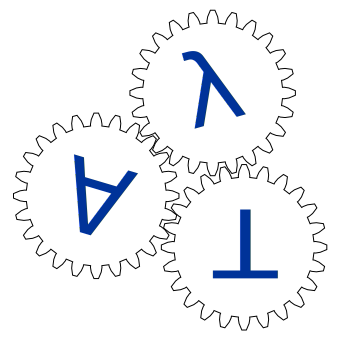
\includegraphics[keepaspectratio,width=5cm]{logo}

\vspace*{20mm}

{\Huge User Manual}

\vspace*{20mm}

{\Large \today}

\vspace*{20mm}

\hrule
\end{center}

\end{titlepage}

\listoffixmes

\tableofcontents
\vfill
\pagebreak

\section{Introduction}

GAPT is a generic architecture for proof transformations implemented in Scala.
Formulas, terms, and other expressions are are represented as lambda terms in
simple type theory.  Terms and formulas of first-order logic and schematic
first-order logic are hence encoded as lambda terms, these form regular
subsets.

The focus of GAPT are proof transformations (in contrast to proof assistants,
whose focus is proof formalization, and automated deduction systems, whose focus
is proof search). GAPT is used from a shell that provides access to the functionality
in the system in a way that is inspired by computer algebra systems: the basic
objects are formulas and (different kinds of) proofs which can be modified
by calling GAPT commands from the command line. In addition, there
is a graphical user interface that allows the user to view (and—to a certain extent—
modify) proofs in a flexible and visually appealing way.

The current functionality of GAPT includes data structures for formulas,
sequents, resolution proofs, sequent calculus proofs, expansion tree proofs
and algorithms for e.g.\ unification, proof skolemization, cut elimination,
cut elimination by resolution~\cite{Baaz00CutElimination}, cut introducton~\cite{Hetzl2012}, etc.

\section{System Requirements}
\label{sec:sysreq}

To run GAPT you need to have Java 7 (or higher) installed.

GAPT contains interfaces to the following automated reasoning systems. Installing
them is optional. If GAPT does not find the executables in the path, the
functionality of these systems will not be available. 

\begin{itemize}
\item Prover9 (\url{http://www.cs.unm.edu/~mccune/mace4/download/}) - make sure
  the commands \texttt{prover9} and \texttt{prooftrans} are available.
\item E theorem prover (\url{http://eprover.org/})
\item LeanCoP (\url{http://leancop.de/})
\item VeriT (\url{http://www.verit-solver.org/})
\item Z3 (\url{https://github.com/Z3Prover/z3})
\item MiniSAT (\url{http://minisat.se/})
\item Glucose (\url{http://www.labri.fr/perso/lsimon/glucose/})
\item Sat4J (\url{http://sat4j.org/})
\item OpenWBO (\url{http://sat.inesc-id.pt/open-wbo/})
\item CVC4 (\url{http://cvc4.cs.nyu.edu/web/})
\end{itemize}

\section{Downloading and Running}

There are three ways you can obtain GAPT:

\begin{enumerate}

\item {\bfseries The recommended way:}  You can download a package of the current
version of GAPT at~\url{https://logic.at/gapt/}.  After extracting
the \texttt{tar.gz}-file, you will find a shell script \texttt{cli.sh}.

Running this script will start the command line interface of GAPT:
\begin{lstlisting}
./cli.sh
\end{lstlisting}

\item If you are adventurous, you can also download an unstable development
  version from github:
\begin{lstlisting}
git clone https://github.com/gapt/gapt
cd gapt
sbt console
\end{lstlisting}

\item If you like GAPT and want to use it as a library in your Scala project,
  it is available as a Maven artificat on JCenter.  All you need to do is add
  one line to your \verb,build.sbt,:
\begin{lstlisting}
libraryDependencies += "at.logic.gapt" %% "gapt" % "1.10"
\end{lstlisting}

\end{enumerate}

The command line interface of GAPT is an interactive Scala shell.  This means
that all functionality of Scala is available to you.  In particular it is easy
to write Scala scripts that use the functionality of GAPT.

You don't need to know anything about Scala to try out the examples in this
manual, but if you do want to learn more about Scala we recommend the book
``Programming in Scala''\cite{odersky2008programming}.

Interactions with the Scala shell are typeset in the following way:
\begin{clilisting}
gapt> println("Hello, world!")
Hello, world!

\end{clilisting}
Here, {\bfseries \cli{println("Hello, world!")}} is the user input, and \texttt{Hello,
world!} is the output from the Scala shell.

If you want to consult the in-depth API documentation of a function, you can
use the \cli{help} command:
\begin{clilisting}
gapt> help(containsQuantifierOnLogicalLevel)

\end{clilisting}

\section{Entering Formulas}\label{sec.entering_formulas}
You can enter formulas by parsing them with the prover9\cite{Prover9Input} parser:
%
\begin{clilisting}
gapt> val H = parseFormula( "(all x (P(x,f(x)) -> (exists y P(x,y))))" )
H: at.logic.gapt.expr.FOLFormula = ∀x.(P(x,f(x))⊃∃y.P(x,y))

\end{clilisting}
%
The prover9 syntax was also extended to higher-order logic, where type declarations are added:
%
\begin{clilisting}
gapt> val I = HLKHOLParser.parseFormula ( "var P:o>i>o; const f:o>i; var x:o; var y:i; (all x (P(x,f(x))) -> (exists y P(x,y)))" )
I: at.logic.gapt.expr.HOLFormula = ∀x:o.(P(x,f(x))⊃∃y.P(x,y))

\end{clilisting}

Please refere to Appendix~\ref{app:formulasyntax} for a full description of the languages the parsers accept.

A collection of formula sequences can be found in the file \cli{examples/FormulaSequences.scala}.
Have a look at this code to see how to compose formulas without the parser.
You can generate instances of these formula sequences by entering, e.g.,
%
\begin{clilisting}
gapt> val f = BussTautology( 5 )
f: at.logic.gapt.proofs.HOLSequent = ((((((c_1∨d_1)∧(c_2∨d_2))∧(c_3∨d_3))∧(c_4∨d_4))⊃c_5)∨(((((c_1∨d_1)∧(c_2∨d_2))∧(c_3∨d_3))∧(c_4∨d_4))⊃d_5)), (((((c_1∨d_1)∧(c_2∨d_2))∧(c_3∨d_3))⊃c_4)∨((((c_1∨d_1)∧(c_2∨d_2))∧(c_3∨d_3))⊃d_4)), ((((c_1∨d_1)∧(c_2∨d_2))⊃c_3)∨(((c_1∨d_1)∧(c_2∨d_2))⊃d_3)), (((c_1∨d_1)⊃c_2)∨((c_1∨d_1)⊃d_2)), (c_1∨d_1) :- c_5, d_5

\end{clilisting}



\section{Automated Deduction}
  
\subsection{SAT Solving}
%
The following shows an example session, using the Sat4j SAT solver
to verify valdity and satisfiability, and query the thus obtained models.
Consider the {\em pigeon hole principle for $(m, n)$, $\mathrm{PHP}_{m,n}$}, which states that if $m$ pigeons
are put into $n$ holes, then there is a hole which contains two pigeons. It is valid
iff $m>n$. $\neg\mathrm{PHP}_{m,n}$ states that when putting $m$ pigeons into $n$ holes, there
is no hole containing two pigeons. This is satisfiable iff $m\leq n$.
\begin{clilisting}
gapt> Sat4j isValid PigeonHolePrinciple(3, 2)
res2: Boolean = true

\end{clilisting}
shows that $\mathrm{PHP}_{3,2}$ is valid, and
\begin{clilisting}
gapt> Sat4j isValid PigeonHolePrinciple(3, 3)
res3: Boolean = false

\end{clilisting}
shows that $\mathrm{PHP}_{3,3}$ is not valid.
Furthermore,
\begin{clilisting}
gapt> val Some(m) = Sat4j solve -PigeonHolePrinciple(3, 3)
m: at.logic.gapt.models.Interpretation =
R(p_1,h_1) -> false
R(p_1,h_2) -> false
R(p_1,h_3) -> true
R(p_2,h_1) -> true
R(p_2,h_2) -> false
R(p_2,h_3) -> false
R(p_3,h_1) -> false
R(p_3,h_2) -> true
R(p_3,h_3) -> false

\end{clilisting}
yields a model of $\neg\mathrm{PHP}_{3,3}$ that can be queried:
\begin{clilisting}
gapt> val p1 = PigeonHolePrinciple.atom(1, 1)
p1: at.logic.gapt.expr.FOLAtom = R(p_1,h_1)

gapt> val p2 = PigeonHolePrinciple.atom(2, 1)
p2: at.logic.gapt.expr.FOLAtom = R(p_2,h_1)

gapt> m.interpret(p1) // Is pigeon 1 in hole 1?
res4: Boolean = false

gapt> m.interpret(p2) // Is pigeon 2 in hole 1?
res5: Boolean = true

\end{clilisting}
We can also interpret quantifier-free formulas:
\begin{clilisting}
gapt> m.interpret( And(p1, p2) )
res6: Boolean = false

\end{clilisting}

We can also convert $\neg\mathrm{PHP}_{3,3}$ into DIMACS format:
\begin{clilisting}
gapt> val (cnf, _, _) = structuralCNF(-PigeonHolePrinciple(3,3), generateJustifications=false, propositional=true)
cnf: Set[at.logic.gapt.proofs.HOLClause] = Set( :- R(p_3,h_1), R(p_3,h_2), R(p_3,h_3), R(p_3,h_2), R(p_2,h_2) :- , R(p_2,h_3), R(p_1,h_3) :- , R(p_3,h_3), R(p_2,h_3) :- ,  :- R(p_2,h_1), R(p_2,h_2), R(p_2,h_3), R(p_3,h_3), R(p_1,h_3) :- , R(p_2,h_1), R(p_1,h_1) :- , R(p_3,h_2), R(p_1,h_2) :- , R(p_3,h_1), R(p_1,h_1) :- , R(p_3,h_1), R(p_2,h_1) :- , R(p_2,h_2), R(p_1,h_2) :- ,  :- R(p_1,h_1), R(p_1,h_2), R(p_1,h_3))

gapt> val encoding = new DIMACSEncoding
encoding: at.logic.gapt.formats.dimacs.DIMACSEncoding = DIMACSEncoding()

gapt> writeDIMACS(encoding encodeCNF cnf)
res7: String =
"p cnf 9 12
1 2 3 0
-2 -4 0
-5 -6 0
-3 -5 0
7 4 5 0
-3 -6 0
-7 -8 0
-2 -9 0
-1 -8 0
-1 -7 0
-4 -9 0
8 9 6 0
"

\end{clilisting}

If you want to know which variable in the DIMACS output corresponds to which
atom in GAPT, you can query the \cli{DIMACSEncoding} object:
\begin{clilisting}
gapt> encoding decodeAtom 1
res8: at.logic.gapt.expr.HOLAtom = R(p_3,h_1)

\end{clilisting}

GAPT also supports other SAT solvers such as MiniSAT or Glucose out of the box:
\begin{clilisting}[MiniSAT.isInstalled]
gapt> MiniSAT isValid PigeonHolePrinciple(3,2)
res9: Boolean = true

\end{clilisting}
\begin{clilisting}[Glucose.isInstalled]
gapt> Glucose isValid PigeonHolePrinciple(3,2)
res10: Boolean = true

\end{clilisting}

If you have another DIMACS-compliant solver installed or want to pass extra
options to the SAT solver, you can pass a custom command to GAPT as well:
\begin{clilisting}[MiniSAT.isInstalled]
gapt> val solver = new ExternalSATSolver("minisat", "-no-pre")
solver: at.logic.gapt.provers.sat.ExternalSATSolver = ExternalSATSolver("minisat", "-no-pre")

gapt> solver isValid PigeonHolePrinciple(3,2)
res11: Boolean = true

\end{clilisting}

\subsection{MaxSAT}

The MaxSAT interface supports generating optimal solutions for weighted partial
MaxSAT instances: these consist of a list of hard clauses, which must be
satisfied in the solution; and a list of weighted soft clauses, where weight of
the satisified soft clauses must be maximized.  See \cite{Argelich2008First}
for an overview.

Let us solve a simple example using the MaxSAT solver from SAT4J:

\begin{clilisting}
gapt> val Seq(a,b,c) = Seq("a","b","c") map {FOLAtom(_)}
a: at.logic.gapt.expr.FOLAtom = a
b: at.logic.gapt.expr.FOLAtom = b
c: at.logic.gapt.expr.FOLAtom = c

gapt> MaxSat4j.solve(hard = a|b|c, soft = Seq(-a -> 4, -b -> 3))
res12: Option[at.logic.gapt.models.Interpretation] =
Some(a -> false
b -> false
c -> true)

\end{clilisting}

GAPT also supports other MaxSAT solvers out of the box, just write
\cli{OpenWBO} or \cli{ToySolver} instead of \cli{MaxSat4j}.

\subsection{SMT Solving}

The SMT solver interface in GAPT supports validity queries for \verb,QF_UF,
formulas.  For example we can check whether a quantifier-free formula is a
quasi-tautology using veriT:
\begin{clilisting}
gapt> val f = parseFormula("(a=b | a=c) & P(c) & P(b) -> P(a)")
f: at.logic.gapt.expr.FOLFormula = (((a=b∨a=c)∧(P(c)∧P(b)))⊃P(a))

\end{clilisting}

\begin{clilisting}[VeriT.isInstalled]
gapt> VeriT isValid f
res13: Boolean = true

\end{clilisting}

GAPT also supports Z3 and CVC4 out of the box (if they are installed):
\begin{clilisting}[Z3.isInstalled && CVC4.isInstalled]
gapt> Z3 isValid f
res10: Boolean = true

gapt> CVC4 isValid f
res11: Boolean = true

\end{clilisting}

You can export \verb,QF_UF, formulas (or sequents) as SMT-LIB benchmarks;
note that we apply a drastic renaming to the constant symbols in order to
support arbitrary (even Unicode) names in GAPT:
\begin{clilisting}
gapt> val (benchmark, typeRenaming, constantRenaming) =                                 SmtLibExporter(Sequent() :+ f)
benchmark: String =
"(set-logic QF_UF)
(declare-sort t1 0)
(declare-fun f1 (t1) Bool)
(declare-fun f2 () t1)
(declare-fun f3 () t1)
(declare-fun f4 () t1)
(assert (not (=> (and (or (= f4 f2) (= f4 f3)) (and (f1 f3) (f1 f2))) (f1 f4))))
(check-sat)
"
typeRenaming: Map[at.logic.gapt.expr.TBase,at.logic.gapt.expr.TBase] = Map(o -> Bool, i -> t1)
constantRenaming: Map[at.logic.gapt.expr.Const,at.logic.gapt.expr.Const] = Map(a -> f4, P -> f1, b -> f2, c -> f3)

\end{clilisting}

We can also extract instances for basic equality axioms (reflexivity, symmetry,
and congruences) from veriT's proof output:
\begin{clilisting}[VeriT.isInstalled]
gapt> val Some(expansionSequent) = VeriT getExpansionSequent (Sequent() :+ f)
expansionSequent: at.logic.gapt.proofs.expansionTrees.ExpansionSequent = WeakQuantifier(∀x.∀y.(x=y⊃y=x), ArrayBuffer((WeakQuantifier(∀y.(a=y⊃y=a), ArrayBuffer((Atom(a=b)⊃Atom(b=a),b), (Atom(a=c)⊃Atom(c=a),c))),a))), WeakQuantifier(∀x1.∀y1.((x1=y1∧P(x1))⊃P(y1)), ArrayBuffer((WeakQuantifier(∀y1.((c=y1∧P(c))⊃P(y1)), ArrayBuffer((Atom(c=a)∧Atom(P(c))⊃Atom(P(a)),a))),c), (WeakQuantifier(∀y1.((b=y1∧P(b))⊃P(y1)), ArrayBuffer((Atom(b=a)∧Atom(P(b))⊃Atom(P(a)),a))),b))) :- Atom(a=b)∨Atom(a=c)∧Atom(P(c))∧Atom(P(b))⊃Atom(P(a))

gapt> extractInstances(expansionSequent) foreach println
(a=b⊃b=a)
(a=c⊃c=a)
((c=a∧P(c))⊃P(a))
((b=a∧P(b))⊃P(a))
(((a=b∨a=c)∧(P(c)∧P(b)))⊃P(a))

\end{clilisting}

\subsection{First-order Theorem Proving}

GAPT includes interfaces to several first-order theorem provers, such as
Prover9, E prover, and LeanCoP.  For Prover9 and E prover we can read back
resolution proofs, and construct LK and expansion proofs from them.  The
LeanCoP interface only supports expansion sequent extraction.

Here is how you can get all of these kinds of proofs using Prover9:
\begin{clilisting}
gapt> val sequent = existsclosure("p(0)" +: "p(x) -> p(s(x))" +: Sequent()                                 :+ "p(s(s(0)))" map parseFormula)
sequent: at.logic.gapt.proofs.HOLSequent = p(0), ∀x.(p(x)⊃p(s(x))) :- p(s(s(0)))

\end{clilisting}

\begin{clilisting}[Prover9.isInstalled]
gapt> Prover9 isValid sequent
res17: Boolean = true

gapt> Prover9 getRobinsonProof sequent
res18: Option[at.logic.gapt.proofs.resolution.ResolutionProof] =
Some([p11]  :-     (Resolution(p10, Suc(0), p9, Ant(0)))
[p10]  :- p(s(0))    (Resolution(p8, Suc(0), p7, Ant(0)))
[p9] p(s(0)) :-     (Resolution(p6, Suc(0), p5, Ant(0)))
[p8]  :- p(0)    (Instance(p4, Substitution()))
[p7] p(0) :- p(s(0))    (Instance(p3, Substitution(v0 -> 0)))
[p6] p(s(0)) :- p(s(s(0)))    (Instance(p3, Substitution(v0 -> s(0))))
[p5] p(s(s(0))) :-     (Instance(p2, Substitution()))
[p4]  :- p(0)    (InputClause( :- p(0)))
[p3] p(v0) :- p(s(v0))    (Instance(p1, Substitution(x -> v0)))
[p2] p(s(s(0))) :-     (InputClause(p(s(s(0))) :- ))
[p1] p(x) :- p(s(x))    (InputClause(p(x) :- p(s(x))))
)

gapt> Prover9 getLKProof sequent
res19: Option[at.logic.gapt.proofs.lkNew.LKProof] =
Some([p19] ∀x.(p(x)⊃p(s(x))), p(0) :- p(s(s(0)))    (ContractionLeftRule(p18, Ant(2), Ant(1)))
[p18] p(0), ∀x.(p(x)⊃p(s(x))), ∀x.(p(x)⊃p(s(x))) :- p(s(s(0)))    (CutRule(p17, Suc(0), p16, Ant(1)))
[p17] p(0), ∀x.(p(x)⊃p(s(x))) :- p(s(0))    (CutRule(p15, Suc(0), p14, Ant(1)))
[p16] ∀x.(p(x)⊃p(s(x))), p(s(0)) :- p(s(s(0)))    (CutRule(p13, Suc(0), p12, Ant(0)))
[p15] p(0) :- p(0)    (ContractionLeftRule(p11, Ant(0), Ant(1)))
[p14] ∀x.(p(x)⊃p(s(x))), p(0) :- p(s(0))    (ContractionLeftRule(p10, Ant(0), Ant(1)))
[p13] ∀x.(p(x)⊃p(s(x))), p(s(0)) :- p(s(s(0)))    (ContractionLeftRule(p9, Ant(0), Ant(1)))
[p12] p(s(s(0))) :- p(s(s(0)))    (ContractionRightRule(p8, Suc(0), Suc(1)))
[p11] p(0), p(0) :- p(0)    (WeakeningLeftRule(p7, p(0)))
[p1...
gapt> Prover9 getExpansionSequent sequent
res20: Option[at.logic.gapt.proofs.expansionTrees.ExpansionSequent] = Some(Atom(p(0)), WeakQuantifier(∀x.(p(x)⊃p(s(x))), List((Atom(p(0))⊃Atom(p(s(0))),0), (Atom(p(s(0)))⊃Atom(p(s(s(0)))),s(0)))) :- Atom(p(s(s(0)))))

\end{clilisting}

All of the above works with E prover as well, we will just show
\cli{getLKProof} as an example:
\begin{clilisting}[EProver.isInstalled]
gapt> EProver getLKProof sequent
res21: Option[at.logic.gapt.proofs.lkNew.LKProof] =
Some([p19] p(0), ∀x.(p(x)⊃p(s(x))) :- p(s(s(0)))    (CutRule(p18, Suc(0), p17, Ant(1)))
[p18] p(0) :- p(0)    (ContractionLeftRule(p16, Ant(0), Ant(1)))
[p17] ∀x.(p(x)⊃p(s(x))), p(0) :- p(s(s(0)))    (ContractionLeftRule(p15, Ant(2), Ant(0)))
[p16] p(0), p(0) :- p(0)    (WeakeningLeftRule(p14, p(0)))
[p15] ∀x.(p(x)⊃p(s(x))), p(0), ∀x.(p(x)⊃p(s(x))) :- p(s(s(0)))    (CutRule(p13, Suc(0), p12, Ant(1)))
[p14] p(0) :- p(0)    (LogicalAxiom(p(0)))
[p13] ∀x.(p(x)⊃p(s(x))), p(0) :- p(s(0))    (ContractionLeftRule(p11, Ant(0), Ant(1)))
[p12] ∀x.(p(x)⊃p(s(x))), p(s(0)) :- p(s(s(0)))    (CutRule(p10, Suc(0), p9, Ant(0)))
[p11] ∀x.(p(x)⊃p(s(x))), ∀x.(p(x)⊃p(s(x))), p(0) :- p(s(0))    (WeakeningLeftRule(p8, ∀x.(p(x)⊃p(s(x)))))
[p10] ∀x.(p(x)⊃p(s(x...
\end{clilisting}

Note that \cli{getLKProof} only works for sequents without strong quantifiers
(i.e.\ sequents that are already Skolemized); however \cli{getExpansionSequent}
will happily return expansion sequents with Skolem quantifiers in that case:
\begin{clilisting}[Prover9.isInstalled]
gapt> val strong = ("(exists x all y P(x,y))" +: Sequent()                                     :+ "(all y exists x P(x,y))" map parseFormula)
strong: at.logic.gapt.proofs.Sequent[at.logic.gapt.expr.FOLFormula] = ∃x.∀y.P(x,y) :- ∀y.∃x.P(x,y)

gapt> Prover9 getExpansionSequent strong
res22: Option[at.logic.gapt.proofs.expansionTrees.ExpansionSequent] = Some(SkolemQuantifier(∃x.∀y.P(x,y), s_{0}, WeakQuantifier(∀y.P(s_{0},y), List((Atom(P(s_{0},s_{2})),s_{2})))) :- SkolemQuantifier(∀y.∃x.P(x,y), s_{2}, WeakQuantifier(∃x.P(x,s_{2}), List((Atom(P(s_{0},s_{2})),s_{0})))))

\end{clilisting}

The LeanCoP interface only supports the \cli{getExpansionSequent} method with
exactly one formula in the succedent:
\begin{clilisting}[LeanCoP.isInstalled]
gapt> LeanCoP getExpansionSequent sequent map {toDeep(_)}
res23: Option[at.logic.gapt.proofs.HOLSequent] = Some(p(0), ((p(0)⊃p(s(0)))∧(p(s(0))⊃p(s(s(0))))) :- p(s(s(0))))

\end{clilisting}

You can also export sequents in TPTP format if you want to pass them to other
provers manually:
\begin{clilisting}
gapt> TPTPFOLExporter.tptp_proof_problem_split(sequent)
res24: String =
"fof( formula0, axiom, 'p'('0') ).
fof( formula1, axiom, (! [X0] : ( 'p'(X0) => 'p'('s'(X0)) )) ).
fof( formula2, conjecture, 'p'('s'('s'('0'))) ).
"

\end{clilisting}

\subsection{Built-In Tableaux Prover}

GAPT contains a  built-in tableaux prover for propositional logic
which can be called with the command \texttt{solve.solvePropositional}, for example as in:
\begin{clilisting}
gapt> solve.solvePropositional(parseFormula("a -> (b -> a&b)"))
res25: Option[at.logic.gapt.proofs.lkNew.LKProof] =
Some([p5]  :- (a⊃(b⊃(a∧b)))    (ImpRightRule(p4, Ant(0), Suc(0)))
[p4] a :- (b⊃(a∧b))    (ImpRightRule(p3, Ant(1), Suc(0)))
[p3] a, b :- (a∧b)    (AndRightRule(p2, Suc(0), p1, Suc(0)))
[p2] a :- a    (LogicalAxiom(a))
[p1] b :- b    (LogicalAxiom(b))
)

\end{clilisting}

\section{Entering Proofs}\label{sec:entering_proofs}

There are various possibilities for entering proofs into the system. The most
basic one is a direct top-down proof-construction using the constructors
of the inference rules.
\begin{clilisting}
gapt> val A = FOLAtom("A")
A: at.logic.gapt.expr.FOLAtom = A

gapt> val B = FOLAtom("B")
B: at.logic.gapt.expr.FOLAtom = B

gapt> val F1 = B --> (A & B)
F1: at.logic.gapt.expr.FOLFormula = (B⊃(A∧B))

gapt> val F2 = A & B
F2: at.logic.gapt.expr.FOLFormula = (A∧B)

\end{clilisting}
%
We start with the axioms:
%
\begin{clilisting}
gapt> val p1 = LogicalAxiom(A)
p1: at.logic.gapt.proofs.lkNew.LogicalAxiom =
[p1] A :- A    (LogicalAxiom(A))

gapt> val p2 = LogicalAxiom(B)
p2: at.logic.gapt.proofs.lkNew.LogicalAxiom =
[p1] B :- B    (LogicalAxiom(B))

\end{clilisting}
%
These are joined by an $\land:\mathrm{right}$-inference. See Appendix~\ref{app:sequent_calculus}
for the formal definition of the sequent calculus used in GAPT.
\begin{clilisting}
gapt> val p3 = AndRightRule( p1, A, p2, B )
p3: at.logic.gapt.proofs.lkNew.AndRightRule =
[p3] A, B :- (A∧B)    (AndRightRule(p2, Suc(0), p1, Suc(0)))
[p2] A :- A    (LogicalAxiom(A))
[p1] B :- B    (LogicalAxiom(B))

\end{clilisting}
%
To finish the proof it remains to apply two $\impl:\mathrm{right}$-inferences:
%
\begin{clilisting}
gapt> val p4 = ImpRightRule( p3, B, F2 )
p4: at.logic.gapt.proofs.lkNew.ImpRightRule =
[p4] A :- (B⊃(A∧B))    (ImpRightRule(p3, Ant(1), Suc(0)))
[p3] A, B :- (A∧B)    (AndRightRule(p2, Suc(0), p1, Suc(0)))
[p2] A :- A    (LogicalAxiom(A))
[p1] B :- B    (LogicalAxiom(B))

gapt> val p5 = ImpRightRule( p4, A, F1 )
p5: at.logic.gapt.proofs.lkNew.ImpRightRule =
[p5]  :- (A⊃(B⊃(A∧B)))    (ImpRightRule(p4, Ant(0), Suc(0)))
[p4] A :- (B⊃(A∧B))    (ImpRightRule(p3, Ant(1), Suc(0)))
[p3] A, B :- (A∧B)    (AndRightRule(p2, Suc(0), p1, Suc(0)))
[p2] A :- A    (LogicalAxiom(A))
[p1] B :- B    (LogicalAxiom(B))

\end{clilisting}
%
You can now view this proof by typing:
\begin{clilisting}
gapt> prooftool( p5 )

\end{clilisting}

The system comes with a collection of example proof sequences in the file
\cli{examples/ProofSequences.scala} which are generated in the above style.
Have a look at this code for more complicated proof constructions.

\section{Proof Theory}

\subsection{Cut-Elimination (Gentzen's method)}

The GAPT-system contains an implementation of reductive cut-elimination
\`{a} la Gentzen. It can be used as follows: first we load a proof p
with cuts (as in Appendix~\ref{sec.fileio}).
%
\begin{clilisting}
gapt> val p = lkOld2New(XMLProofDatabaseParser( "examples/simple/fol1.xml.gz" ).proofs(0)._2)
p: at.logic.gapt.proofs.lkNew.LKProof =
[p25] ∀x.∀y.(P(x,y)⊃Q(x,y)) :- ∃x.∃y.(¬Q(x,y)⊃¬P(x,y))    (CutRule(p24, Suc(0), p23, Ant(0)))
[p24] ∀x.∀y.(P(x,y)⊃Q(x,y)) :- ∀x.∃y.(¬P(x,y)∨Q(x,y))    (ForallRightRule(p22, Suc(0), z, x))
[p23] ∀x.∃y.(¬P(x,y)∨Q(x,y)) :- ∃x.∃y.(¬Q(x,y)⊃¬P(x,y))    (ForallLeftRule(p21, Ant(0), ∃y.(¬P(x,y)∨Q(x,y)), b, x))
[p22] ∀x.∀y.(P(x,y)⊃Q(x,y)) :- ∃y.(¬P(z,y)∨Q(z,y))    (ExistsRightRule(p20, Suc(0), (¬P(z,y)∨Q(z,y)), a, y))
[p21] ∃y.(¬P(b,y)∨Q(b,y)) :- ∃x.∃y.(¬Q(x,y)⊃¬P(x,y))    (ExistsLeftRule(p19, Ant(0), v, y))
[p20] ∀x.∀y.(P(x,y)⊃Q(x,y)) :- (¬P(z,a)∨Q(z,a))    (ForallLeftRule(p18, Ant(0), ∀y.(P(x,y)⊃Q(x,y)), z, x))
[p19] (¬P(b,v)∨Q(b,v)) :- ∃x.∃y.(¬Q(x,y)⊃¬P(x,y))    (ExistsRightRule(p17, Suc(0), ∃y.(¬Q(x,y)⊃¬P(x,y)), b, x))
[p18] ∀y.(P(z,y)⊃Q(z,y)) :- (¬P(z...
\end{clilisting}
%
and then call the cut-elimination procedure:
\begin{clilisting}
gapt> val q = ReductiveCutElimination( p )
q: at.logic.gapt.proofs.lkNew.LKProof =
[p16] ∀x.∀y.(P(x,y)⊃Q(x,y)) :- ∃x.∃y.(¬Q(x,y)⊃¬P(x,y))    (ForallLeftRule(p15, Ant(0), ∀y.(P(x,y)⊃Q(x,y)), b, x))
[p15] ∀y.(P(b,y)⊃Q(b,y)) :- ∃x.∃y.(¬Q(x,y)⊃¬P(x,y))    (ForallLeftRule(p14, Ant(0), (P(b,y)⊃Q(b,y)), a, y))
[p14] (P(b,a)⊃Q(b,a)) :- ∃x.∃y.(¬Q(x,y)⊃¬P(x,y))    (ContractionRightRule(p13, Suc(0), Suc(1)))
[p13] (P(b,a)⊃Q(b,a)) :- ∃x.∃y.(¬Q(x,y)⊃¬P(x,y)), ∃x.∃y.(¬Q(x,y)⊃¬P(x,y))    (ImpLeftRule(p12, Suc(0), p11, Ant(0)))
[p12]  :- P(b,a), ∃x.∃y.(¬Q(x,y)⊃¬P(x,y))    (ExistsRightRule(p10, Suc(1), ∃y.(¬Q(x,y)⊃¬P(x,y)), b, x))
[p11] Q(b,a) :- ∃x.∃y.(¬Q(x,y)⊃¬P(x,y))    (ExistsRightRule(p9, Suc(0), ∃y.(¬Q(x,y)⊃¬P(x,y)), b, x))
[p10]  :- P(b,a), ∃y.(¬Q(b,y)⊃¬P(b,y))    (ExistsRightRule(p8, Suc(1), (¬Q(b,y)⊃¬P(b,y)), a, y))
[p9] Q(b,a) :- ∃y.(¬...
\end{clilisting}


\subsection{Skolemization}

Skolemization consists of replacing the variables bound by strong quantifiers in the end-sequent of a proof
by new function symbols thus obtaining a validity-equivalent sequent. In the GAPT-system Skolemization
is implemented for proofs and can be used, e.g.~as follows:
%
\begin{clilisting}
gapt> val proofs = XMLProofDatabaseParser( "examples/prime/ceres_xml/prime1-1.xml.gz" ).proofs
proofs: List[(String, at.logic.gapt.proofs.lk.base.LKProof)] = List((the-proof,CutRuleType(PRIME-DIV, REM, PRE, F[1] :- )))

gapt> val p = proofs(0)._2
p: at.logic.gapt.proofs.lk.base.LKProof = CutRuleType(PRIME-DIV, REM, PRE, F[1] :- )

gapt> val q = skolemize( lkOld2New(p) )
q: at.logic.gapt.proofs.lkNew.LKProof =
[p968] F[1], PRIME-DIV, PRE, REM :-     (CutRule(p967, Suc(0), p966, Ant(0)))
[p967] F[1], PRIME-DIV, PRE, REM :- INF(set_1(1))    (CutRule(p965, Suc(0), p964, Ant(4)))
[p966] INF(set_1(1)) :-     (DefinitionLeftRule(p963, Ant(0), INF(set_1(1))))
[p965]  :- ¬empty(set_1(1))    (NegRightRule(p962, Ant(0)))
[p964] F[1], PRIME-DIV, PRE, REM, ¬empty(set_1(1)) :- INF(set_1(1))    (CutRule(p961, Suc(0), p960, Ant(0)))
[p963] ∀m.∃n.∈((m+(n+1)),set_1(1)) :-     (ForallLeftRule(p959, Ant(0), ∃n.∈((m+(n+1)),set_1(1)), 1, m))
[p962] empty(set_1(1)) :-     (DefinitionLeftRule(p958, Ant(0), empty(set_1(1))))
[p961] F[1], PRIME-DIV, PRE, REM :- O(set_1(1))    (CutRule(p957, Suc(0), p956, Ant(0)))
[p960] O(set_1(1)), ¬empty(set_1(1)) :- INF(set_1(1))    (CutRule...
\end{clilisting}


\subsection{Interpolation}

\fxwarning{Use a more reasonable example here.}

The command \texttt{ExtractInterpolant} extracts an interpolant from a sequent calculus proof which may contain atomic cuts and/or equality rules. Currently, we allow only reflexivity axioms or axioms of the form $A \seq A$. The implementation is based on Lemma 6.5 of~\cite{Takeuti87Proof}. The method expects
a proof p and an arbitrary partition of the end-sequent $\Gamma \seq \Delta$ of p into a 
``negative part'' $\Gamma_1\seq\Delta_1$ and a ``positive part'' $\Gamma_2 \seq \Delta_2$.
It returns a formula $I$ s.t.\ $\Gamma_1\seq\Delta_1, I$ and $I,\Gamma_2\seq\Delta_2$
are provable and $I$ contains only such predicate symbols that appear in both, $\Gamma_1\seq\Delta_1$
and $\Gamma_2\seq\Delta_2$. For example, suppose pr is a proof of $p \lor q \seq p, q$
by a single $\lor$-left inference (see Section~\ref{sec:entering_proofs} for how to construct
such a proof), then you can compute an interpolant as follows:
\begin{clilisting}
gapt> val pr: LKProof = p3
pr: at.logic.gapt.proofs.lkNew.LKProof =
[p3] A, B :- (A∧B)    (AndRightRule(p2, Suc(0), p1, Suc(0)))
[p2] A :- A    (LogicalAxiom(A))
[p1] B :- B    (LogicalAxiom(B))

gapt> val I = ExtractInterpolant(pr, Seq(Ant(0), Suc(0)), Seq(Ant(1)))
I: at.logic.gapt.expr.HOLFormula = (⊥∨¬B)

\end{clilisting}

\subsection{Expansion Trees}

Expansion trees are a compact representation of cut-free proofs. They have originally been
introduced in~\cite{Miller87Compact}. GAPT contains an implementation of
expansion trees for higher-order logic including functions for extracting expansion
trees from proofs, for merging expansion trees, for pruning and transforming them
in various ways and for viewing them in a comfortable way in the graphical user interface.

An expansion tree contains the instances of the quantifiers for a formula. In order
to represent an LK-proof we use {\em expansion sequents}, i.e.~sequents of expansion trees.
We can obtain an expansion sequent for example by:
\begin{clilisting}
gapt> val p = SquareEdgesExampleProof( 4 )
p: at.logic.gapt.proofs.lkNew.LKProof =
[p40] ∀x.∀y.(P(x,y)⊃P(s(x),y)), P(0,0), ∀x.∀y.(P(x,y)⊃P(x,s(y))) :- P(s(s(s(s(0)))),s(s(s(s(0)))))    (ContractionLeftRule(p39, Ant(0), Ant(2)))
[p39] ∀x.∀y.(P(x,y)⊃P(s(x),y)), P(0,0), ∀x.∀y.(P(x,y)⊃P(s(x),y)), ∀x.∀y.(P(x,y)⊃P(x,s(y))) :- P(s(s(s(s(0)))),s(s(s(s(0)))))    (ForallLeftRule(p38, Ant(0), ∀y.(P(x,y)⊃P(s(x),y)), 0, x))
[p38] ∀y.(P(0,y)⊃P(s(0),y)), P(0,0), ∀x.∀y.(P(x,y)⊃P(s(x),y)), ∀x.∀y.(P(x,y)⊃P(x,s(y))) :- P(s(s(s(s(0)))),s(s(s(s(0)))))    (ForallLeftRule(p37, Ant(0), (P(0,y)⊃P(s(0),y)), 0, y))
[p37] (P(0,0)⊃P(s(0),0)), P(0,0), ∀x.∀y.(P(x,y)⊃P(s(x),y)), ∀x.∀y.(P(x,y)⊃P(x,s(y))) :- P(s(s(s(s(0)))),s(s(s(s(0)))))    (ImpLeftRule(p36, Suc(0), p35, Ant(1)))
[p36] P(0,0) :- P(0,0)    (LogicalAxiom(P(0,0)))
[p35] ∀x.∀y.(P(x,y)⊃P(s(x),y)), P...
gapt> val E = LKToExpansionProof( p )
E: at.logic.gapt.proofs.expansionTrees.ExpansionSequent = WeakQuantifier(∀x.∀y.(P(x,y)⊃P(s(x),y)), List((WeakQuantifier(∀y.(P(0,y)⊃P(s(0),y)), List((Atom(P(0,0))⊃Atom(P(s(0),0)),0))),0), (WeakQuantifier(∀y.(P(s(0),y)⊃P(s(s(0)),y)), List((Atom(P(s(0),0))⊃Atom(P(s(s(0)),0)),0))),s(0)), (WeakQuantifier(∀y.(P(s(s(0)),y)⊃P(s(s(s(0))),y)), List((Atom(P(s(s(0)),0))⊃Atom(P(s(s(s(0))),0)),0))),s(s(0))), (WeakQuantifier(∀y.(P(s(s(s(0))),y)⊃P(s(s(s(s(0)))),y)), List((Atom(P(s(s(s(0))),0))⊃Atom(P(s(s(s(s(0)))),0)),0))),s(s(s(0)))))), Atom(P(0,0)), WeakQuantifier(∀x.∀y.(P(x,y)⊃P(x,s(y))), List((WeakQuantifier(∀y.(P(s(s(s(s(0)))),y)⊃P(s(s(s(s(0)))),s(y))), List((Atom(P(s(s(s(s(0)))),0))⊃Atom(P(s(s(s(s(0)))),s(0))),0), (Atom(P(s(s(s(s(0)))),s(0)))⊃Atom(P(s(s(s(s(0)))),s(s(0)))),s(0)), (Atom(P(s(s(s(s(...
\end{clilisting}
This expansion sequent can then be viewed in the graphical user interface by simply calling:
\begin{clilisting}
gapt> prooftool( E )

\end{clilisting}
Prooftool is then intialized with displaying the end-sequent of \cli{p}, i.e.\ the shallow sequent
of \cli{E}. The user can then selectively expand quantifiers by clicking on them, see~\cite{Hetzl13Understanding}
for a detailed description.


\section{Cut-Elimination by Resolution (CERES)}

\subsection{First-Order Logic}

\fxnote{The ceres-functionality should be demonstrated by an short example}

\subsection{Higher-Order Logic}

\fxnote{TODO}

\section{Cut-Introduction}

The cut-introduction algorithm as described in~\cite{Hetzl2012,Hetzl14Algorithmic,Hetzl14Introducing} is
implemented in GAPT for introducing $\Pi_1$-cuts into a sequent calculus
proof. We will use as input one of the proofs generated by
the system, namely, \texttt{LinearExampleProof(9)}. But the user can also
write his own proofs (see Section~\ref{sec:entering_proofs})
and input them to the cut-introduction algorithm.

Take an example proof:
\begin{clilisting}
gapt> val p = LinearExampleProof(4)
p: at.logic.gapt.proofs.lkNew.LKProof =
[p18] ∀x.(P(x)⊃P(s(x))), P(0) :- P(s(s(s(s(0)))))    (ContractionLeftRule(p17, Ant(0), Ant(2)))
[p17] ∀x.(P(x)⊃P(s(x))), P(0), ∀x.(P(x)⊃P(s(x))) :- P(s(s(s(s(0)))))    (ForallLeftRule(p16, Ant(0), (P(x)⊃P(s(x))), 0, x))
[p16] (P(0)⊃P(s(0))), P(0), ∀x.(P(x)⊃P(s(x))) :- P(s(s(s(s(0)))))    (ImpLeftRule(p15, Suc(0), p14, Ant(1)))
[p15] P(0) :- P(0)    (LogicalAxiom(P(0)))
[p14] ∀x.(P(x)⊃P(s(x))), P(s(0)) :- P(s(s(s(s(0)))))    (ContractionLeftRule(p13, Ant(0), Ant(2)))
[p13] ∀x.(P(x)⊃P(s(x))), P(s(0)), ∀x.(P(x)⊃P(s(x))) :- P(s(s(s(s(0)))))    (ForallLeftRule(p12, Ant(0), (P(x)⊃P(s(x))), s(0), x))
[p12] (P(s(0))⊃P(s(s(0)))), P(s(0)), ∀x.(P(x)⊃P(s(x))) :- P(s(s(s(s(0)))))    (ImpLeftRule(p11, Suc(0), p10, Ant(1)))
[p11] P(s(0)) :- P(s(0))    (LogicalAx...
\end{clilisting}
Then compute a proof with a single cut that contains a single quantifier by:
\begin{clilisting}
gapt> val q = CutIntroduction.compressLKProof( p,                                   DeltaTableMethod( manyQuantifiers=false ), verbose=true )
Total inferences in the input proof: 16
Quantifier inferences in the input proof: 4
End sequent: ∀x.(P(x)⊃P(s(x))), P(0) :- P(s(s(s(s(0)))))
Size of term set: 6
Smallest grammar of size 6:
Axiom: (τ)
Non-terminal vectors:
  (τ)
  (α_0)
Productions:
  τ -> -{P(0)}_a1

  τ -> -{∀x.(P(x)⊃P(s(x)))}_a0(s(α_0))

  τ -> -{∀x.(P(x)⊃P(s(x)))}_a0(α_0)

  τ -> {P(s(s(s(s(0)))))}_s0

  α_0 -> 0

  α_0 -> s(s(0))


Size of the canonical solution: 8
Size of the minimized solution: 4
CNF of minimized cut-formula number 0:
  P(α_0) :- P(s(s(α_0)))
Number of cuts introduced: 1
Total inferences in the proof with cut(s): 19
Quantifier inferences in the proof with cut(s): 5
q: Option[at.logic.gapt.proofs.lkNew.LKProof] =
Some([p19] ∀x.(P(x)⊃P(s(x))), P(0) :- P(s(s(s(s(0)))))    (CutRule(p18, Suc(0), p17, Ant(0)))
[p18] ∀x.(P(x)⊃P(s(x))) :- ∀α_0.(P(α_0)⊃P(s(s(α_0))))    (ForallRightRule(p16, Suc(0), α_0, α_0))
[p17] ∀α_0.(P(α_0)⊃P(s(s(α_0)))), P(0) :- P(s(s(s(s(0)))))    (ContractionLeftRule(p15, Ant(1), Ant(0)))
[p16] ∀x.(P(x)⊃P(s(x))) :- (P(α_0)⊃P(s(s(α_0))))    (ContractionLeftRule(p14, Ant(1), Ant(0)))
[p15] ∀α_0.(P(α_0)⊃P(s(s(α_0)))), ∀α_0.(P(α_0)⊃P(s(s(α_0)))), P(0) :- P(s(s(s(s(0)))))    (ForallLeftRule(p13, Ant(2), (P(α_0)⊃P(s(s(α_0)))), s(s(0)), α_0))
[p14] ∀x.(P(x)⊃P(s(x))), ∀x.(P(x)⊃P(s(x))) :- (P(α_0)⊃P(s(s(α_0))))    (ForallLeftRule(p12, Ant(1), (P(x)⊃P(s(x))), s(α_0), x))
[p13] ∀α_0.(P(α_0)⊃P(s(s(α_0)))), P(0), (P(s(s(0)))⊃P(s(s(s(s(0)))))) :-...
\end{clilisting}
You can also try \texttt{DeltaTableMethod(manyQuantifiers=true)}, this will proceed as above but will
compute a single cut with a block of quantifiers.  The method \texttt{MaxSATMethod(1,2)}
uses a reduction to a MaxSAT problem and an external MaxSAT-solver for finding a
minimal grammar corresponding to a proof with a cut with two cuts, one with $1$
quantifer, one with $2$ quantifers.

\section{Tree grammars}

\fxnote{Give grammar minimization example}

\vfill
\pagebreak
\begin{appendix}

\section{Proof systems}

\subsection{LK}\label{app:sequent_calculus}

The rules of LK are listed below. Proof trees are constructed top-down, starting with axioms and with each rule introducing new inferences. With the exception of the definition rules, the constructors of the rules only allow inferences that are actually valid. Note that the rules are presented here as if they always act upon the outermost formulas in the upper sequent, but this is only for convenience of presentation. The basic constructors actually require the user to specify on which concrete formulas the inference should be performed.

Apart from those basic constructors, there is also a multitude of convenience constructors that facilitate easier proof construction. Moreover, there are so-called macro rules that reduce several inferences to a single command (e.g. introducing quantifier blocks). See the API documentation of the individual rules for details. 

\subsubsection*{Axioms}

\begin{multicols}{2}
\begin{prooftree}
\AxiomCm{}
\RightLabelm{(\mt{Logical axiom})}
\UnaryInfCm{A \seq A}
\end{prooftree}

\begin{prooftree}
\AxiomCm{}
\RightLabelm{\mt{$\top$ axiom}}
\UnaryInfCm{\seq \top}
\end{prooftree}

\begin{prooftree}
\AxiomCm{}
\RightLabelm{(\mt{Reflexivity axiom})}
\UnaryInfCm{\seq t = t}
\end{prooftree}

\begin{prooftree}
\AxiomCm{}
\RightLabelm{\mt{$\bot$ axiom}}
\UnaryInfCm{\bot \seq}
\end{prooftree}
\end{multicols}

\begin{prooftree}
\AxiomCm{}
\RightLabelm{\mt{Theory axiom}}
\UnaryInfCm{\Gamma \seq \Delta}
\end{prooftree}

Logical axioms and theory axioms may only contain atomic formulas.

\subsubsection*{Cut}

  \begin{prooftree}
  \AxiomCm{\Gamma \seq \Delta, A}
  \AxiomCm{A, \Sigma \seq \Pi}
  \RightLabelm{(\mt{cut})}
  \BinaryInfCm{\Gamma, \Sigma \seq \Delta, \Pi}
  \end{prooftree}

\subsubsection*{Structural rules}

\begin{multicols}{2}

  \subsubsection*{Left rules}
  
  \begin{prooftree}
  \AxiomCm{\Gamma \seq \Delta}
  \RightLabelm{(\mt{w:l})}
  \UnaryInfCm{A, \Gamma \seq \Delta}
  \end{prooftree}
  
  \begin{prooftree}
  \AxiomCm{A,A,\Gamma \seq \Delta}
  \RightLabelm{(\mt{c:l})}
  \UnaryInfCm{A,\Gamma\seq \Delta}
  \end{prooftree}
  
  \subsubsection*{Right rules}
  
  \begin{prooftree}
  \AxiomCm{\Gamma \seq \Delta}
  \RightLabelm{(\mt{w:r})}
  \UnaryInfCm{\Gamma \seq \Delta, A}
  \end{prooftree}
  
  \begin{prooftree}
  \AxiomCm{\Gamma \seq \Delta, A, A}
  \RightLabelm{(\mt{c:r})}
  \UnaryInfCm{\Gamma \seq \Delta, A}
  \end{prooftree}

\end{multicols}

\newpage

\subsubsection*{Propositional rules}

\begin{multicols}{2}

  \subsubsection*{Left rules}

  \begin{prooftree}
  \AxiomCm{A,B,\Gamma \seq \Delta}
  \RightLabelm{(\land\mt{:l})}
  \UnaryInfCm{A \land B,\Gamma \seq \Delta}
  \end{prooftree}
  
  \begin{prooftree}
  \AxiomCm{A, \Gamma \seq \Delta}
  \AxiomCm{B, \Sigma \seq \Pi}
  \RightLabelm{(\lor\mt{:l})}
  \BinaryInfCm{A \lor B, \Gamma, \Sigma \seq \Delta, \Pi}
  \end{prooftree}
  
  \begin{prooftree}
  \AxiomCm{\Gamma \seq \Delta, A}
  \RightLabelm{(\lnot\mt{:l})}
  \UnaryInfCm{\neg A, \Gamma \seq \Delta}
  \end{prooftree}
  
  \begin{prooftree}
  \AxiomCm{\Gamma \seq \Delta, A}
  \AxiomCm{B, \Sigma \seq \Pi}
  \RightLabelm{(\impl\mt{:l})}
  \BinaryInfCm{A \impl B, \Gamma, \Sigma \seq \Delta, \Pi}
  \end{prooftree}

  \subsubsection*{Right rules}

  \begin{prooftree}
  \AxiomCm{\Gamma \seq \Delta, A}
  \AxiomCm{\Sigma \seq \Pi, B}
  \RightLabelm{(\land\mt{:r})}
  \BinaryInfCm{\Gamma, \Sigma \seq \Delta, \Pi, A \land B}
  \end{prooftree}
  
  \begin{prooftree}
  \AxiomCm{\Gamma \seq \Delta, A, B}
  \RightLabelm{(\lor\mt{:r})}
  \UnaryInfCm{\Gamma \seq \Delta, A \lor B}
  \end{prooftree}
  
  \begin{prooftree}
  \AxiomCm{A, \Gamma\seq \Delta}
  \RightLabelm{(\lnot\mt{:r})}
  \UnaryInfCm{\Gamma \seq \Delta, \neg A}
  \end{prooftree}
  
  \begin{prooftree}
  \AxiomCm{A, \Gamma \seq \Delta, B}
  \RightLabelm{(\impl\mt{:r})}
  \UnaryInfCm{\Gamma \seq \Delta, A \impl B}
  \end{prooftree}

\end{multicols}

\subsubsection*{Quantifier rules}

\begin{multicols}{2}

  \subsubsection*{Left rules}

  \begin{prooftree}
  \AxiomCm{A[t/x], \Gamma \seq \Delta}
  \RightLabelm{(\forall\mt{:l})}
  \UnaryInfCm{\forall x A, \Gamma \seq \Delta}
  \end{prooftree}
  
  \begin{prooftree}
  \AxiomCm{ A[y/x], \Gamma \seq \Delta}
  \RightLabelm{(\exists\mt{:l})}
  \UnaryInfCm{\exists x A, \Gamma \seq \Delta}
  \end{prooftree}
  
  \subsubsection*{Right rules}
  
  \begin{prooftree}
  \AxiomCm{\Gamma \seq \Delta, A[y/x]}
  \RightLabelm{(\forall\mt{:r})}
  \UnaryInfCm{\Gamma \seq \Delta, \forall x A}
  \end{prooftree}
  
  \begin{prooftree}
  \AxiomCm{\Gamma \seq \Delta, A[t/x]}
  \RightLabelm{(\exists\mt{:r})}
  \UnaryInfCm{\Gamma \seq \Delta, \exists x A}
  \end{prooftree}

\end{multicols}

The variable $y$ must not occur free in $\Gamma$, $\Delta$ or $A$. The term $t$ must avoid variable capture, i.e. it must not contain free occurrences of variables bound in $A$.

\subsubsection*{Equality rules}

\begin{multicols}{2}

  \subsubsection*{Left rules}

  \begin{prooftree}
  \AxiomCm{s = t, A[T/s], \Sigma \seq \Pi}
  \RightLabelm{(\mt{=:l})}
  \UnaryInfCm{s = t, A[T/t], \Sigma \seq \Pi}
  \end{prooftree}
  
  \begin{prooftree}
  \AxiomCm{s = t, A[T/t], \Sigma \seq \Pi}
  \RightLabelm{(\mt{=:l})}
  \UnaryInfCm{s = t, A[T/s], \Sigma \seq \Pi}
  \end{prooftree}
  
  \subsubsection*{Right rules}
  
  \begin{prooftree}
  \AxiomCm{s = t, \Sigma \seq \Pi, A[T/s]}
  \RightLabelm{(\mt{=:r})}
  \UnaryInfCm{s = t, \Sigma \seq \Pi, A[T/t]}
  \end{prooftree}
  
  \begin{prooftree}
  \AxiomCm{s = t, \Sigma \seq \Pi, A[T/t]}
  \RightLabelm{(\mt{=:r})}
  \UnaryInfCm{s = t, \Sigma \seq \Pi, A[T/s]}
  \end{prooftree}
  
\end{multicols}
Each equation rule replaces exactly one occurrence of a term in its auxiliary formula.

\subsubsection*{Definition rules}
\begin{center}
 \AxiomCm{A, \Gamma \seq \Delta}
 \RightLabelm{(\mt{def:l})}
 \UnaryInfCm{B, \Gamma \seq \Delta}
 \DisplayProof
 \AxiomCm{\Gamma \seq \Delta, A}
 \RightLabelm{(\mt{def:r})}
 \UnaryInfCm{\Gamma \seq \Delta, B}
 \DisplayProof
\end{center}
These definition rules are extremely liberal, as they allow the replacement of any formula by any other formula.

\subsubsection*{Induction}
  The induction rule applies to arbitrary algebraic datatypes. Let $c_1,...,c_n$ be the constructors of a type and let $k_i$ be the arity of $c_i$. Let $F[x]$ be a formula with $x$ a free variable of the appropriate type. Then we call the sequent $\mathcal{S}_i := F[x_1],...,F[x_{k_i}], \Gamma_i \seq \Delta_i, F[c_i(x_1,...,x_{k_i})]$ the $i$-th induction step. In this case, the induction rule has the form
  \begin{prooftree}
    \AxiomCm{(\pi_1)}
    \noLine
    \UnaryInfCm{\mathcal{S}_1}
    \AxiomCm{(\pi_2)}
    \noLine
    \UnaryInfCm{\mathcal{S}_2}
    \AxiomCm{\dots}
    \AxiomCm{(\pi_n)}
    \noLine
    \UnaryInfCm{\mathcal{S}_n}
    \RightLabelm{(\mt{ind})}
    \QuaternaryInfC{$\Gamma \seq \Delta, \forall x F[x]$}
  \end{prooftree}
  
  In the case of the natural numbers, there are two constructors: $0$ of arity 0 and $s$ of arity 1. Consequently, the induction rule reduces to
  
  \begin{prooftree}
    \AxiomCm{(\pi_1)}
    \noLine
    \UnaryInfCm{\Gamma_1 \seq \Delta_1, F[0]}
    \AxiomCm{(\pi_2)}
    \noLine
    \UnaryInfCm{F[x], \Gamma_2 \seq \Delta_2, F[sx]}
    \RightLabelm{(\mt{ind})}
    \BinaryInfCm{\Gamma_1, \Gamma_2 \seq \Delta_1, \Delta_2, \forall x F[x]}
  \end{prooftree}

\subsection{Resolution}

\subsection*{Initial clauses}

\begin{prooftree}
\AxiomC{}\RightLabel{InputClause}
\UnaryInfC{$C$}
\end{prooftree}

\begin{prooftree}
\AxiomC{}\RightLabel{ReflexivityClause}
\UnaryInfC{$t=t$}
\end{prooftree}

\begin{prooftree}
\AxiomC{}\RightLabel{TautologyClause}
\UnaryInfC{$a \lor \neg a$}
\end{prooftree}

\subsection*{Structural rules}

\begin{prooftree}
\AxiomC{$a \lor a \lor C$}\RightLabel{Factor}
\UnaryInfC{$a \lor C$}
\end{prooftree}

\begin{prooftree}
\AxiomC{$C$}\RightLabel{Instance}
\UnaryInfC{$C \sigma$}
\end{prooftree}

\subsection*{Logical rules}

\begin{prooftree}
\AxiomC{$C \lor a$}
\AxiomC{$\neg a \lor D$}
\RightLabel{Resolution}
\BinaryInfC{$C \lor D$}
\end{prooftree}

\begin{prooftree}
\AxiomC{$C \lor t=s$}
\AxiomC{$l[t] \lor D$}
\RightLabel{Paramodulation}
\BinaryInfC{$C \lor l[s] \lor D$}
\end{prooftree}

\begin{prooftree}
\AxiomC{$C \lor t=s$}
\AxiomC{$l[s] \lor D$}
\RightLabel{Paramodulation}
\BinaryInfC{$C \lor l[t] \lor D$}
\end{prooftree}

\subsection{LKsk}

LKsk is a sequent calculus used in the CERES method for higher-order logic, see
\cite{Weller2010CERES} for an overview of both the calculus and the method.

LKsk operates on labelled formulas. A label $\ell$ is a finite list of terms, a labelled formula is a pair $(F, \ell)$, written as $\sklabel{F}{\ell}$. If $\ell$ is a label and $t$ a term, we write $\ell;t$ for the concatenation of $\ell$ and $t$.

\subsubsection*{Axioms}

\begin{multicols}{2}
\begin{prooftree}
\AxiomCm{}
\RightLabelm{(\mt{Logical axiom})}
\UnaryInfCm{\sklabel{A}{\ell_1} \seq \sklabel{A}{\ell_2}}
\end{prooftree}

\begin{prooftree}
\AxiomCm{}
\RightLabelm{\mt{$\top$ axiom}}
\UnaryInfCm{\seq \sklabel{\top}{\ell}}
\end{prooftree}

\begin{prooftree}
\AxiomCm{}
\RightLabelm{(\mt{Reflexivity axiom})}
\UnaryInfCm{\seq \sklabel{t = t}{\ell}}
\end{prooftree}

\begin{prooftree}
\AxiomCm{}
\RightLabelm{\mt{$\bot$ axiom}}
\UnaryInfCm{\sklabel{\bot}{\ell}\seq}
\end{prooftree}
\end{multicols}

\begin{prooftree}
\AxiomCm{}
\RightLabelm{\mt{Theory axiom}}
\UnaryInfCm{\sklabel{A_1}{\ell_1},...,\sklabel{A_m}{\ell_m} \seq \sklabel{B_1}{\ell'_1},...,\sklabel{B_n}{\ell'_n}}
\end{prooftree}

Logical axioms and theory axioms may only contain atomic formulas.

\subsubsection*{Cut}

  \begin{prooftree}
  \AxiomCm{\Gamma \seq \Delta, \sklabel{A}{\ell_1}}
  \AxiomCm{\sklabel{A}{\ell_2}, \Sigma \seq \Pi}
  \RightLabelm{(\mt{cut})}
  \BinaryInfCm{\Gamma, \Sigma \seq \Delta, \Pi}
  \end{prooftree}
  
  Note that the labels of the cut formulas do not need to be equal.

\subsubsection*{Structural rules}

\begin{multicols}{2}

  \subsubsection*{Left rules}
  
  \begin{prooftree}
  \AxiomCm{\Gamma \seq \Delta}
  \RightLabelm{(\mt{w:l})}
  \UnaryInfCm{\sklabel{A}{\ell}, \Gamma \seq \Delta}
  \end{prooftree}
  
  \begin{prooftree}
  \AxiomCm{\sklabel{A}{\ell},\sklabel{A}{\ell},\Gamma \seq \Delta}
  \RightLabelm{(\mt{c:l})}
  \UnaryInfCm{\sklabel{A}{\ell},\Gamma\seq \Delta}
  \end{prooftree}
  
  \subsubsection*{Right rules}
  
  \begin{prooftree}
  \AxiomCm{\Gamma \seq \Delta}
  \RightLabelm{(\mt{w:r})}
  \UnaryInfCm{\Gamma \seq \Delta, \sklabel{A}{\ell}}
  \end{prooftree}
  
  \begin{prooftree}
  \AxiomCm{\Gamma \seq \Delta, \sklabel{A}{\ell}, \sklabel{A}{\ell}}
  \RightLabelm{(\mt{c:r})}
  \UnaryInfCm{\Gamma \seq \Delta, \sklabel{A}{\ell}}
  \end{prooftree}

\end{multicols}

\subsubsection*{Propositional rules}

\begin{multicols}{2}

  \subsubsection*{Left rules}

  \begin{prooftree}
  \AxiomCm{\sklabel{A}{\ell},\sklabel{B}{\ell},\Gamma \seq \Delta}
  \RightLabelm{(\land\mt{:l})}
  \UnaryInfCm{\sklabel{A \land B}{\ell},\Gamma \seq \Delta}
  \end{prooftree}
  
  \begin{prooftree}
  \AxiomCm{\sklabel{A}{\ell}, \Gamma \seq \Delta}
  \AxiomCm{\sklabel{B}{\ell}, \Sigma \seq \Pi}
  \RightLabelm{(\lor\mt{:l})}
  \BinaryInfCm{\sklabel{A \lor B}{\ell}, \Gamma, \Sigma \seq \Delta, \Pi}
  \end{prooftree}
  
  \begin{prooftree}
  \AxiomCm{\Gamma \seq \Delta, \sklabel{A}{\ell}}
  \RightLabelm{(\lnot\mt{:l})}
  \UnaryInfCm{\sklabel{\neg A}{\ell}, \Gamma \seq \Delta}
  \end{prooftree}
  
  \begin{prooftree}
  \AxiomCm{\Gamma \seq \Delta, \sklabel{A}{\ell}}
  \AxiomCm{\sklabel{B}{\ell}, \Sigma \seq \Pi}
  \RightLabelm{(\impl\mt{:l})}
  \BinaryInfCm{\sklabel{A \impl B}{\ell}, \Gamma, \Sigma \seq \Delta, \Pi}
  \end{prooftree}

  \subsubsection*{Right rules}

  \begin{prooftree}
  \AxiomCm{\Gamma \seq \Delta, \sklabel{A}{\ell}}
  \AxiomCm{\Sigma \seq \Pi, \sklabel{B}{\ell}}
  \RightLabelm{(\land\mt{:r})}
  \BinaryInfCm{\Gamma, \Sigma \seq \Delta, \Pi, \sklabel{A \land B}{\ell}}
  \end{prooftree}
  
  \begin{prooftree}
  \AxiomCm{\Gamma \seq \Delta, \sklabel{A}{\ell}, \sklabel{B}{\ell}}
  \RightLabelm{(\lor\mt{:r})}
  \UnaryInfCm{\Gamma \seq \Delta, \sklabel{A \lor B}{\ell}}
  \end{prooftree}
  
  \begin{prooftree}
  \AxiomCm{\sklabel{A}{\ell}, \Gamma\seq \Delta}
  \RightLabelm{(\lnot\mt{:r})}
  \UnaryInfCm{\Gamma \seq \Delta, \sklabel{\neg A}{\ell}}
  \end{prooftree}
  
  \begin{prooftree}
  \AxiomCm{\sklabel{A}{\ell}, \Gamma \seq \Delta, \sklabel{B}{\ell}}
  \RightLabelm{(\impl\mt{:r})}
  \UnaryInfCm{\Gamma \seq \Delta, \sklabel{A \impl B}{\ell}}
  \end{prooftree}

\end{multicols}

\subsubsection*{Quantifier rules}

\begin{multicols}{2}

  \subsubsection*{Left rules}
  
   \begin{prooftree}
  \AxiomCm{\sklabel{A[t/x]}{\ell;t}, \Gamma \seq \Delta}
  \RightLabelm{(\forall\mt{:l})}
  \UnaryInfCm{\sklabel{\forall x A}{\ell}, \Gamma \seq \Delta}
  \end{prooftree}
  
  \begin{prooftree}
  \AxiomCm{ \sklabel{A[y/x]}{\ell}, \Gamma \seq \Delta}
  \RightLabelm{(\exists\mt{:l})}
  \UnaryInfCm{\sklabel{\exists x A}{\ell}, \Gamma \seq \Delta}
  \end{prooftree}
  
  \begin{prooftree}
  \AxiomCm{ \sklabel{A[f(\ell)/x]}{\ell}, \Gamma \seq \Delta}
  \RightLabelm{(\exists^{sk}\mt{:l})}
  \UnaryInfCm{\sklabel{\exists x A}{\ell}, \Gamma \seq \Delta}
  \end{prooftree}
  
  \subsubsection*{Right rules}
  
  \begin{prooftree}
  \AxiomCm{\Gamma \seq \Delta, \sklabel{A[y/x]}{\ell}}
  \RightLabelm{(\forall\mt{:r})}
  \UnaryInfCm{\Gamma \seq \Delta, \sklabel{\forall x A}{\ell}}
  \end{prooftree}
  
  \begin{prooftree}
  \AxiomCm{\Gamma \seq \Delta, \sklabel{A[f(\ell)/x]}{\ell}}
  \RightLabelm{(\forall^{sk}\mt{:r})}
  \UnaryInfCm{\Gamma \seq \Delta, \sklabel{\forall x A}{\ell}}
  \end{prooftree}
  
  \begin{prooftree}
  \AxiomCm{\Gamma \seq \Delta, \sklabel{A[t/x]}{\ell;t}}
  \RightLabelm{(\exists\mt{:r})}
  \UnaryInfCm{\Gamma \seq \Delta, \sklabel{\exists x A}{\ell}}
  \end{prooftree}

\end{multicols}

The variable $y$ must not occur free in $\Gamma$, $\Delta$ or $A$. The term $t$ must avoid variable capture, i.e. it must not contain free occurrences of variables bound in $A$.

\subsubsection*{Equality rules}

\begin{multicols}{2}

  \subsubsection*{Left rules}

  \begin{prooftree}
  \AxiomCm{\sklabel{s = t}{\ell_1}, \sklabel{A[T/s]}{\ell_2}, \Sigma \seq \Pi}
  \RightLabelm{(\mt{=:l})}
  \UnaryInfCm{\sklabel{s = t}{\ell_1}, \sklabel{A[T/t]}{\ell_2}, \Sigma \seq \Pi}
  \end{prooftree}
  
  \begin{prooftree}
  \AxiomCm{\sklabel{s = t}{\ell_1}, \sklabel{A[T/t]}{\ell_2}, \Sigma \seq \Pi}
  \RightLabelm{(\mt{=:l})}
  \UnaryInfCm{\sklabel{s = t}{\ell_1}, \sklabel{A[T/s]}{\ell_2}, \Sigma \seq \Pi}
  \end{prooftree}
  
  \subsubsection*{Right rules}
  
  \begin{prooftree}
  \AxiomCm{\sklabel{s = t}{\ell_1}, \Sigma \seq \Pi, \sklabel{A[T/s]}{\ell_2}}
  \RightLabelm{(\mt{=:r})}
  \UnaryInfCm{\sklabel{s = t}{\ell_1}, \Sigma \seq \Pi, \sklabel{A[T/t]}{\ell_2}}
  \end{prooftree}
  
  \begin{prooftree}
  \AxiomCm{\sklabel{s = t}{\ell_1}, \Sigma \seq \Pi, \sklabel{A[T/t]}{\ell_2}}
  \RightLabelm{(\mt{=:r})}
  \UnaryInfCm{\sklabel{s = t}{\ell_1}, \Sigma \seq \Pi,\sklabel{A[T/s]}{\ell_2}}
  \end{prooftree}
  
\end{multicols}
Each equation rule replaces exactly one occurrence of a term in its auxiliary formula.

\subsection{Ral}

Ral is a higher-order resolution calculus used in the CERES method for
higher-order logic, see again \cite{Weller2010CERES} for details.

Ral operates on sequents of labelled formulas, just as LKsk.  A label $\ell$ is
a finite set of terms, a labelled formula is a pair $(F, \ell)$, written as
$\sklabel{F}{\ell}$. If $\ell$ is a label and $t$ a term, we write $\ell;t$ for
the concatenation of $\ell$ and $t$.

\begin{prooftree}
  \AxiomCm{}
  \RightLabel{RalInitial}
  \UnaryInfCm{\Gamma \vdash \Delta}
\end{prooftree}

The substitution also substitutes the variables in the labels:
\begin{prooftree}
  \AxiomCm{\Gamma \vdash \Delta}
  \RightLabel{RalSub}
  \UnaryInfCm{\Gamma\sigma \vdash \Delta\sigma}
\end{prooftree}

The resolution rule does not require the labels to be equal:
\begin{prooftree}
  \AxiomCm{\Gamma \vdash \Delta, \sklabel{A}{\ell_1}, \dots, \sklabel{A}{\ell_m}}
  \AxiomCm{\sklabel{A}{\ell_1}, \dots, \sklabel{A}{\ell_n}, \Sigma \vdash \Pi}
  \RightLabel{RalCut}
  \BinaryInfCm{\Gamma, \Sigma \vdash \Delta, \Pi}
\end{prooftree}

Factoring is restricted to atoms:
\begin{multicols}{2}
\begin{prooftree}
  \AxiomCm{\sklabel{a}{\ell_1}{a},\sklabel{a}{\ell_2},\Gamma \vdash \Delta}
  \RightLabel{RalFactor}
  \UnaryInfCm{\sklabel{a}{\ell_1}, \Gamma \vdash \Delta}
\end{prooftree}
\begin{prooftree}
  \AxiomCm{\Gamma \vdash \Delta, \sklabel{a}{\ell_1},\sklabel{a}{\ell_2}}
  \RightLabel{RalFactor}
  \UnaryInfCm{\Gamma \vdash \Delta, \sklabel{a}{\ell_1}}
\end{prooftree}
\end{multicols}

Paramodulation can rewrite the equation in both directions, in a formula of the
antecedent or the succedent---this is one of the four possibilities:
\begin{prooftree}
  \AxiomCm{\Gamma \vdash \Delta, \sklabel{t=s}{\ell}}
  \AxiomCm{\Sigma \vdash \Pi, \sklabel{A[t]}{\ell}}
  \RightLabel{RalPara}
  \BinaryInfCm{\Gamma, \Sigma \vdash \Delta, \sklabel{A[s]}{\ell}}
\end{prooftree}

\begin{multicols}{2}
\begin{prooftree}
  \AxiomCm{\sklabel{\forall x\: A[x]}{\ell}, \Gamma \vdash \Delta}
  \RightLabel{RalAllF}
  \UnaryInfCm{\sklabel{A[s\ell]}{\ell}, \Gamma \vdash \Delta}
\end{prooftree}
\begin{prooftree}
  \AxiomCm{\Gamma \vdash \Delta, \sklabel{\forall x\: A[x]}{\ell}}
  \RightLabel{RalAllT}
  \UnaryInfCm{\Gamma \vdash \Delta, \sklabel{A[\alpha]}{\ell;\alpha}}
\end{prooftree}
\end{multicols}

\begin{multicols}{2}
\begin{prooftree}
  \AxiomCm{\sklabel{\exists x\: A[x]}{\ell}, \Gamma \vdash \Delta}
  \RightLabel{RalExF}
  \UnaryInfCm{\sklabel{A[\alpha]}{\ell;\alpha}, \Gamma \vdash \Delta}
\end{prooftree}
\begin{prooftree}
  \AxiomCm{\Gamma \vdash \Delta, \sklabel{\exists x\: A[x]}{\ell}}
  \RightLabel{RalExT}
  \UnaryInfCm{\Gamma \vdash \Delta, \sklabel{A[s\ell]}{\ell}}
\end{prooftree}
\end{multicols}

\begin{multicols}{2}
\begin{prooftree}
  \AxiomCm{\sklabel{\top}{\ell}, \Gamma \vdash \Delta}
  \RightLabel{RalTopF}
  \UnaryInfCm{\Gamma \vdash \Delta}
\end{prooftree}
\begin{prooftree}
  \AxiomCm{\Gamma \vdash \Delta, \sklabel{\bot}{\ell}}
  \RightLabel{RalBottomT}
  \UnaryInfCm{\Gamma \vdash \Delta}
\end{prooftree}
\end{multicols}

\begin{multicols}{2}
\begin{prooftree}
  \AxiomCm{\sklabel{\neg A}{\ell}, \Gamma \vdash \Delta}
  \RightLabel{RalNegF}
  \UnaryInfCm{\Gamma \vdash \Delta, \sklabel{A}{\ell}}
\end{prooftree}
\begin{prooftree}
  \AxiomCm{\Gamma \vdash \Delta, \sklabel{\neg A}{\ell}}
  \RightLabel{RalNegT}
  \UnaryInfCm{\sklabel{A}{\ell}, \Gamma \vdash \Delta}
\end{prooftree}
\end{multicols}

\begin{multicols}{3}
\begin{prooftree}
  \AxiomCm{\sklabel{A \land B}{\ell}, \Gamma \vdash \Delta}
  \RightLabel{RalAndF}
  \UnaryInfCm{\sklabel{A}{\ell}, \sklabel{B}{\ell}, \Gamma \vdash \Delta}
\end{prooftree}
\begin{prooftree}
  \AxiomCm{\Gamma \vdash \Delta, \sklabel{A \land B}{\ell}}
  \RightLabel{RalAndT1}
  \UnaryInfCm{\Gamma \vdash \Delta, \sklabel{A}{\ell}}
\end{prooftree}
\begin{prooftree}
  \AxiomCm{\Gamma \vdash \Delta, \sklabel{A \land B}{\ell}}
  \RightLabel{RalAndT2}
  \UnaryInfCm{\Gamma \vdash \Delta, \sklabel{B}{\ell}}
\end{prooftree}
\end{multicols}

\begin{multicols}{3}
\begin{prooftree}
  \AxiomCm{\sklabel{A \lor B}{\ell}, \Gamma \vdash \Delta}
  \RightLabel{RalOrF1}
  \UnaryInfCm{\sklabel{A}{\ell}, \Gamma \vdash \Delta}
\end{prooftree}
\begin{prooftree}
  \AxiomCm{\sklabel{A \lor B}{\ell}, \Gamma \vdash \Delta}
  \RightLabel{RalOrF2}
  \UnaryInfCm{\sklabel{B}{\ell}, \Gamma \vdash \Delta}
\end{prooftree}
\begin{prooftree}
  \AxiomCm{\Gamma \vdash \Delta, \sklabel{A \lor B}{\ell}}
  \RightLabel{RalOrT}
  \UnaryInfCm{\Gamma \vdash \Delta, \sklabel{A}{\ell}, \sklabel{B}{\ell}}
\end{prooftree}
\end{multicols}

\begin{multicols}{3}
\begin{prooftree}
  \AxiomCm{\sklabel{A \impl B}{\ell}, \Gamma \vdash \Delta}
  \RightLabel{RalImpF1}
  \UnaryInfCm{\Gamma \vdash \Delta, \sklabel{A}{\ell}}
\end{prooftree}
\begin{prooftree}
  \AxiomCm{\sklabel{A \impl B}{\ell}, \Gamma \vdash \Delta}
  \RightLabel{RalImpF2}
  \UnaryInfCm{\sklabel{B}{\ell}, \Gamma \vdash \Delta}
\end{prooftree}
\begin{prooftree}
  \AxiomCm{\Gamma \vdash \Delta, \sklabel{A \impl B}{\ell}}
  \RightLabel{RalImpT}
  \UnaryInfCm{\sklabel{A}{\ell}, \Gamma \vdash \Delta, \sklabel{B}{\ell}}
\end{prooftree}
\end{multicols}

\fxnote{Expansion trees?}

\section{Formula Syntax}
\label{app:formulasyntax}
\subsection{Prover 9 parser (parseFormula)}

The Prover9 parser interpretes names strings built over the alphabet
 $[\mathtt{a, \ldots, z, A ,\ldots, Z, 0, \ldots 9} ]$. Also the
 equality symbol $=$ and the arithmetic operators $\{\mathtt{+,-,*,/}\}$
 are names.

Since prover 9 has two naming schemes, we describe both of them. The default
 is the native LADR scheme.

\subsubsection{LADR naming scheme (default)}

Names starting with lower case letters from \texttt{u} to \texttt{z} are
 interpeted as variable symbols. Every name starting with a different letter
 is interpeted as a constant/function/predicate symbol, depending on the
 position in the term.

\subsubsection{Prolog naming scheme}
Names starting with upper case letters from \texttt{A} to \texttt{Z} are
 interpeted as variable symbols. Every name starting with a different letter
 is interpeted as a constant/function, depending on the
 position in the term. Predicates start with a lower or an upper case letter.

\subsubsection{Terms and Formulas}
Arguments are always seperated by commas and put in parenthesis. Terms are
 built from variable, constant symbols and function symbols applied
 to a number of arguments, which are terms. Likewise, atoms are
 predicate symbols, possibly with arguments which are again terms. The
 function symbols $\{\mathtt{+,-,*,/}\}$ and the equality predicate $=$
 are written in infix notation.

For example, the following are terms in the LADR naming scheme:

 \begin{lstlisting}
   "constant", "variable", "function(constant,variable)", "s_{21} + 5"
 \end{lstlisting}

And the following are atoms:

 \begin{lstlisting}
   "P1(alpha, beta(x))", "25 = v"
 \end{lstlisting}

The logical connectives are called $\{\mathtt{\&,|,->,all,exists}\}$ where
 the quantifiers and negation are written in prefix form and conjunction,
 disjunction and implication are written in infix form.

Conjunction and disjunction are right-associative. Quantifiers always need to
 be enclosed in parenthesis but a series of quantfiers doesn't need parenthesis
 in between. The binding order is (from strongest to weakest):
 $\mathtt{\neg,\forall,\exists,\land\lor,\rightarrow}$.


For example, the formula $\forall x (P(x,f(x)) \rightarrow \exists y P(x,y))$
 is parsed as:

\begin{clilisting}
gapt> parseFormula("(all x (P(x,f(x)) -> (exists y P(x,y))))")
res28: at.logic.gapt.expr.FOLFormula = ∀x.(P(x,f(x))⊃∃y.P(x,y))

\end{clilisting}

The Prolog scheme can be parsed as well using the \texttt{Prover9TermParser}
class:

\begin{clilisting}
gapt> Prover9TermParser.parseFormula("(all X (P(X,f(X)) -> (exists Y P(X,Y))))")
res29: at.logic.gapt.expr.FOLFormula = ∀X.(P(X,f(X))⊃∃Y.P(X,Y))

\end{clilisting}

\section{XML proof parser}\label{sec.fileio}

This method \texttt{XMLProofDatabaseParser} will take as an argument a string that represents the path of a file
containing a proof database in the xml format (generated by HLK, for example) and
will return a proof database containing a list 
of pairs. It expects a file (the string of a proof will not work) and you can use 
the relative path. In the list returned, each pair is composed of a string and 
an object representing a proof within the system. The string is the name of the 
proof defined in the xml file. For example:
%
\begin{clilisting}
gapt> val proofs = XMLProofDatabaseParser( "examples/simple/fol1.xml.gz" ).proofs
proofs: List[(String, at.logic.gapt.proofs.lk.base.LKProof)] = List((p,CutRuleType(∀x.∀y.(P(x,y)⊃Q(x,y)) :- ∃x.∃y.(¬Q(x,y)⊃¬P(x,y)))))

\end{clilisting}
%
returns a list of length 1 as shown by entering
%
\begin{clilisting}
gapt> proofs.length
res30: Int = 1

\end{clilisting}
%
Its only element is \cli{proofs(0)}, the name of this proof can be obtained by
entering
%
\begin{clilisting}
gapt> proofs(0)._1
res31: String = p

\end{clilisting}
%
and the proof itself by
%
\begin{clilisting}
gapt> val proof = lkOld2New(proofs(0)._2)
proof: at.logic.gapt.proofs.lkNew.LKProof =
[p25] ∀x.∀y.(P(x,y)⊃Q(x,y)) :- ∃x.∃y.(¬Q(x,y)⊃¬P(x,y))    (CutRule(p24, Suc(0), p23, Ant(0)))
[p24] ∀x.∀y.(P(x,y)⊃Q(x,y)) :- ∀x.∃y.(¬P(x,y)∨Q(x,y))    (ForallRightRule(p22, Suc(0), z, x))
[p23] ∀x.∃y.(¬P(x,y)∨Q(x,y)) :- ∃x.∃y.(¬Q(x,y)⊃¬P(x,y))    (ForallLeftRule(p21, Ant(0), ∃y.(¬P(x,y)∨Q(x,y)), b, x))
[p22] ∀x.∀y.(P(x,y)⊃Q(x,y)) :- ∃y.(¬P(z,y)∨Q(z,y))    (ExistsRightRule(p20, Suc(0), (¬P(z,y)∨Q(z,y)), a, y))
[p21] ∃y.(¬P(b,y)∨Q(b,y)) :- ∃x.∃y.(¬Q(x,y)⊃¬P(x,y))    (ExistsLeftRule(p19, Ant(0), v, y))
[p20] ∀x.∀y.(P(x,y)⊃Q(x,y)) :- (¬P(z,a)∨Q(z,a))    (ForallLeftRule(p18, Ant(0), ∀y.(P(x,y)⊃Q(x,y)), z, x))
[p19] (¬P(b,v)∨Q(b,v)) :- ∃x.∃y.(¬Q(x,y)⊃¬P(x,y))    (ExistsRightRule(p17, Suc(0), ∃y.(¬Q(x,y)⊃¬P(x,y)), b, x))
[p18] ∀y.(P(z,y)⊃Q(z,y)) :- (...
\end{clilisting}
%
You can then view this proof in the graphical user interface \texttt{prooftool} by 
entering
%
\begin{clilisting}
gapt> prooftool( proof )

\end{clilisting}
%
In the folder \cli{../examples/simple} you can find a number of further simple
proofs.

\end{appendix}

\vfill
\pagebreak

\bibliographystyle{plain}
\bibliography{references}
\end{document}
